\part{Un corpus déjà structuré}

\clearpage
\thispagestyle{empty}
\cleardoublepage
\vspace*{\stretch{0.3}}
Le corpus sur lequel nous avons travaillé est un ensemble de fichiers XML-TEI. Ces derniers résultent d'une version numérisée des \odm{} réalisée et hébergée par le site \ia, elle-même issue du traitement des volumes physiques de l'Université de Toronto. Dans cette première partie, nous allons décrire ces différents états des \odm{} et commenter les opérations qui ont mené à leur structuration, tout en interrogeant les raisons ayant conduit le programme \timeus{} à les privilégier par rapport à d'autre version similaires.ddd
\vspace*{\stretch{1.7}}

\chapter{Un corpus d'imprimés}

\section{Une publication sur une soixantaine d'années}

La publication des trois séries des \odm{} s'échelonne sur soixante-treize années (1857-1930). Les modalités de publication évoluent à partir de 1885  : là  où les monographies de la première série avaient été directement publiées en volume (1857-1885), celles des deuxième (1885-1899) et troisième série (1904-1928) sont publiées sous forme de fascicules trimestriels qui sont ensuite reliés en volumes\footnote{\cite[p. 124]{lorry}.}. Des éléments de paratexte sont également fournis aux relieurs : page de titre, introduction au volume, index, errata et table des matières.

Le passage des volumes reliés aux fascicules trimestriels est annoncé par l'éditeur dans l'\textit{Avertissement} liminaire du premier fascicule de la deuxième série :

\begin{quote}
    \og La nouvelle série des \odm{} s'ouvre avec 
le présent fascicule. Le grand nombre des travaux soumis à la 
Société d'Économie sociale assure l'avenir et la régularité 
de la publication. \textit{Les monographies paraîtront désormais en 
fascicules trimestriels}\footnote{\cite[\og Avertissement \fg{}, p. I]{mono047a}. Nous soulignons.}. \fg{}
\end{quote}

Dans l'\textit{Avertissement} général de ce volume, édité en 1887 et placé immédiatement après la page de titre et le sommaire, le changement est à nouveau annoncé, mais également justifié :

\begin{quote}
    \og Quand la Société d'Économie sociale, en 1882, perdit celui qui 
avait réglé son rôle auprès de lui et après lui\footnote{Frédéric Le Play est mort le 5 avril 1882.}, elle trouva le cinquième tome des \odm{} arrêté au premier tiers de sa publication : elle acheva de le mettre au jour. Puis, voulant laisser bien distincts des travaux accomplis sous l'\oe{}il du maître, ceux dont il lui fallait dès lors prendre seule la responsabilité, \textit{elle commença en juillet 1885, sous le même titre, une nouvelle série de monographies de familles paraissant par fascicules trimestriels}\footnote{\cite[spec. p. II]{s2avert}. Nous soulignons.}. \fg{}
\end{quote}

\begin{figure}[t]
    \centering
    \begin{subfigure}[t]{0.4\textwidth}
     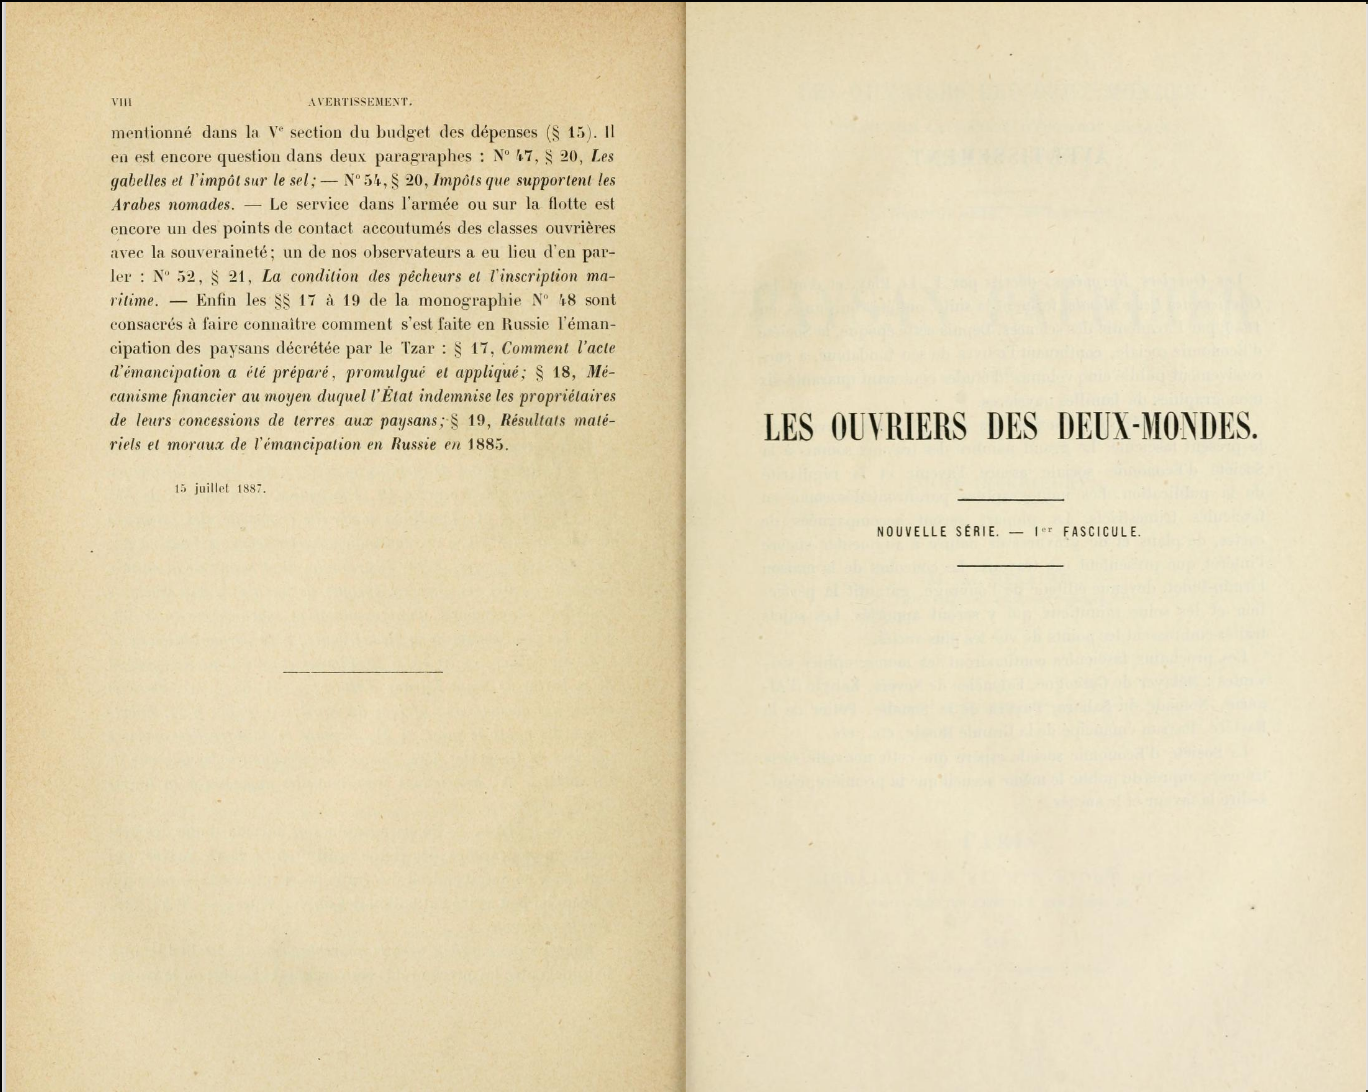
\includegraphics[width=1\linewidth]{img/odm47_ia_1.png}
     \caption{}
     \label{odm47ia1}
    \end{subfigure}
    \hspace{5pt}
    \begin{subfigure}[t]{0.4\textwidth}
     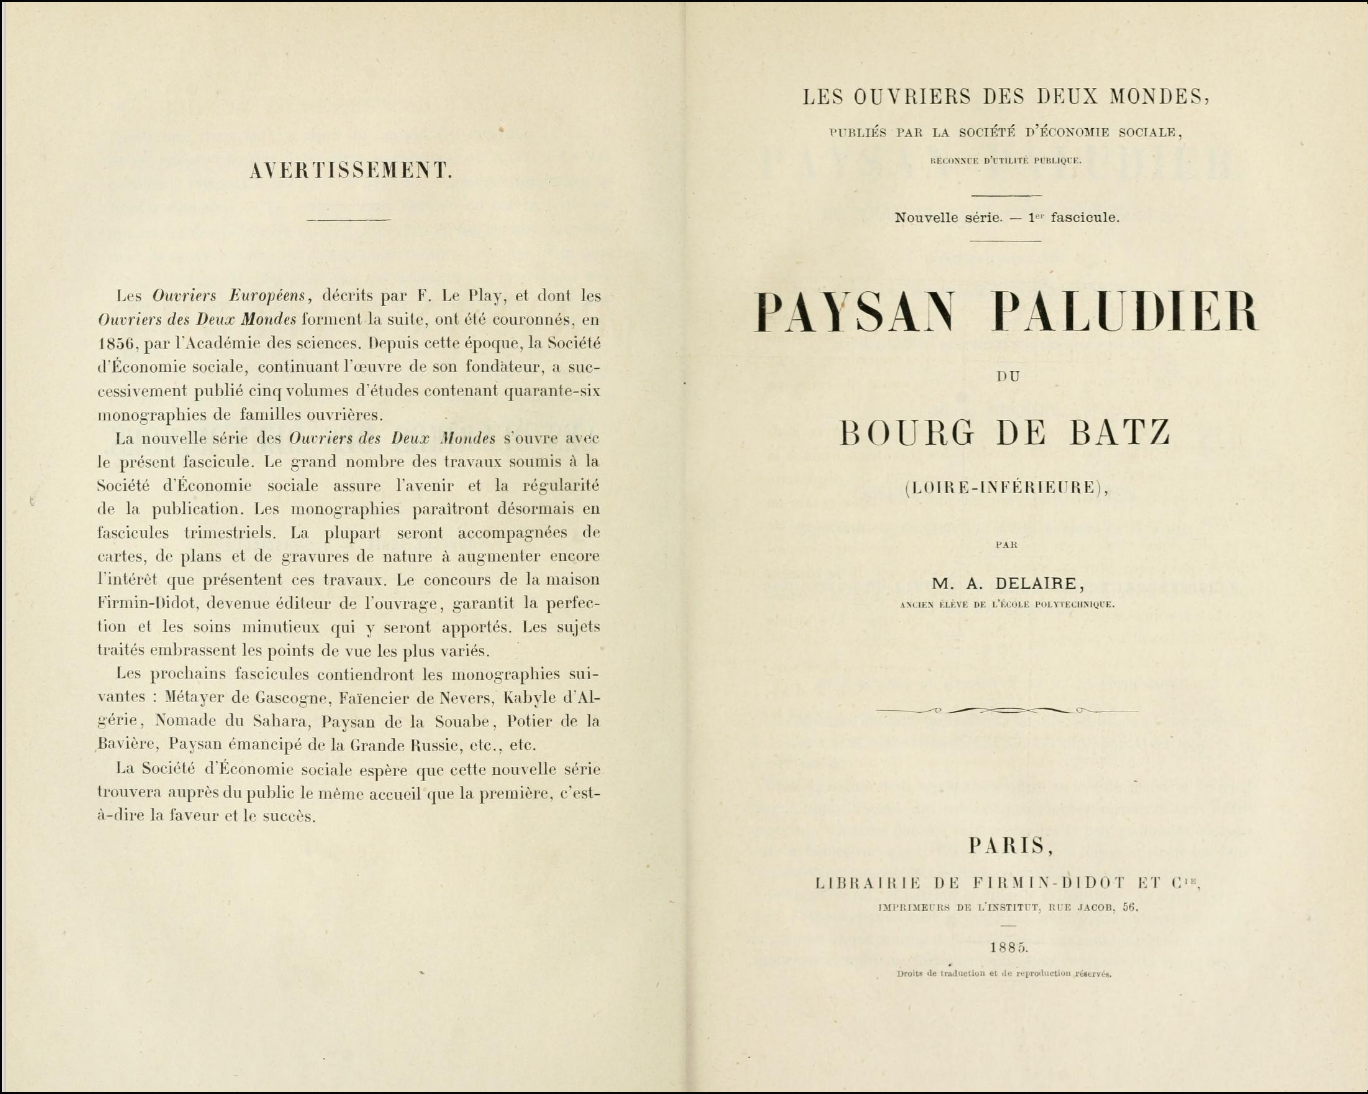
\includegraphics[width=1\linewidth]{img/odm47_ia_2.png}
     \caption{}
     \label{odm47ia2}
    \end{subfigure}
    \hspace{5pt}
    
    
    
    \begin{subfigure}[t]{0.4\textwidth}
     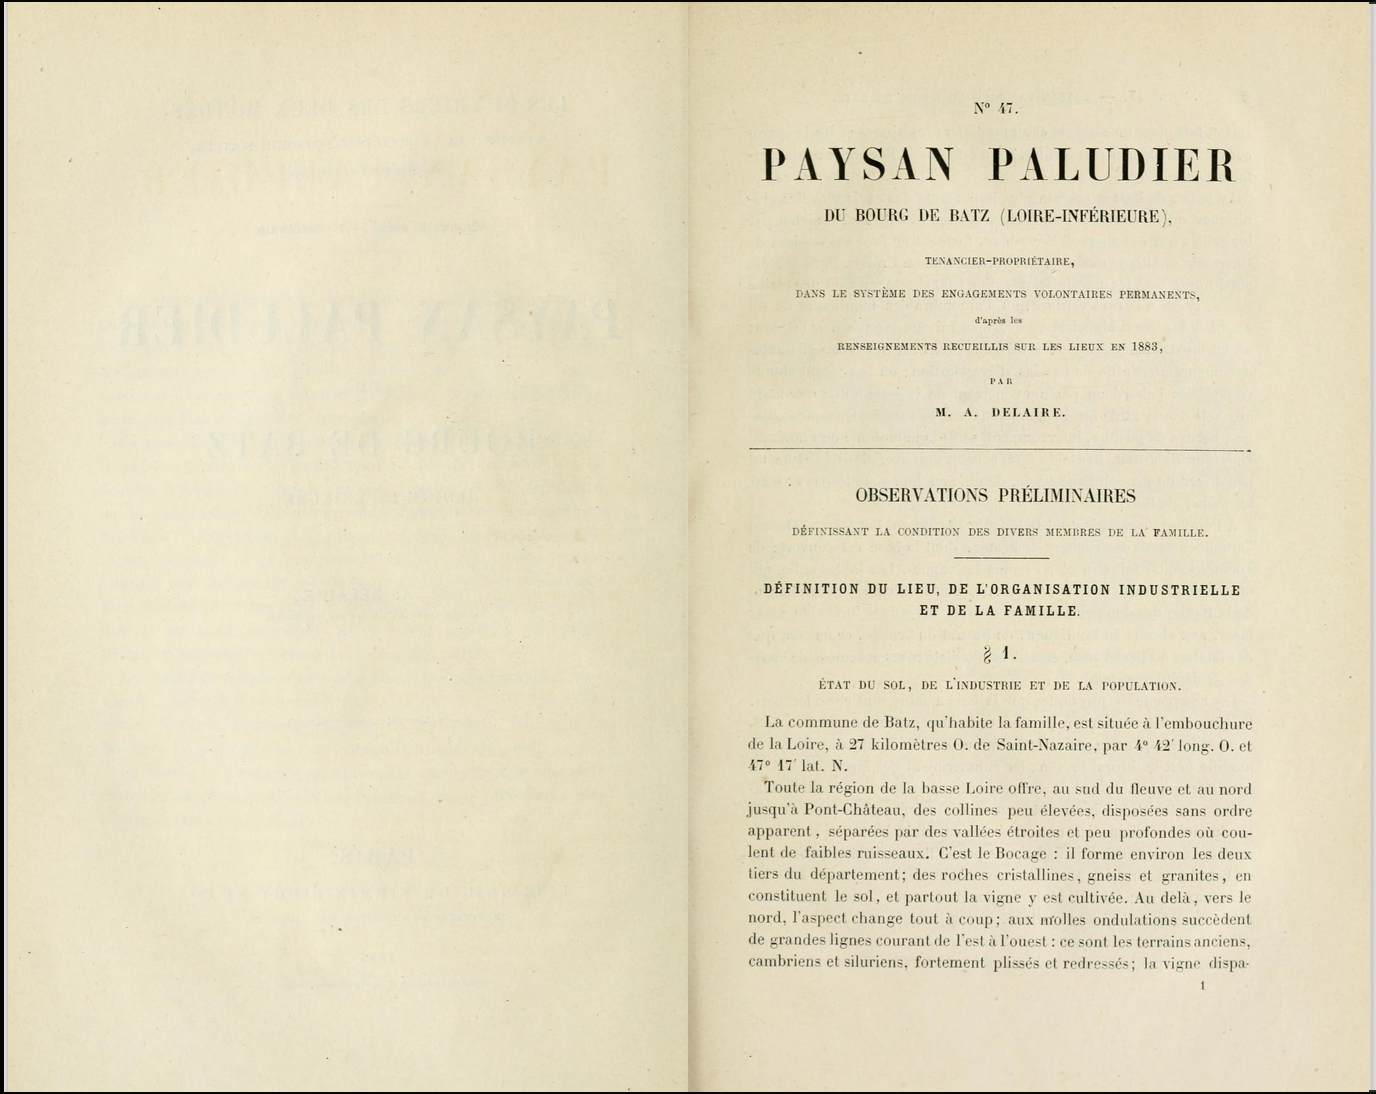
\includegraphics[width=1\linewidth]{img/odm47_ia_3.png}
     \caption{}
     \label{odm47ia3}
    \end{subfigure}
    \hspace{5pt}
    \begin{subfigure}[t]{0.4\textwidth}
     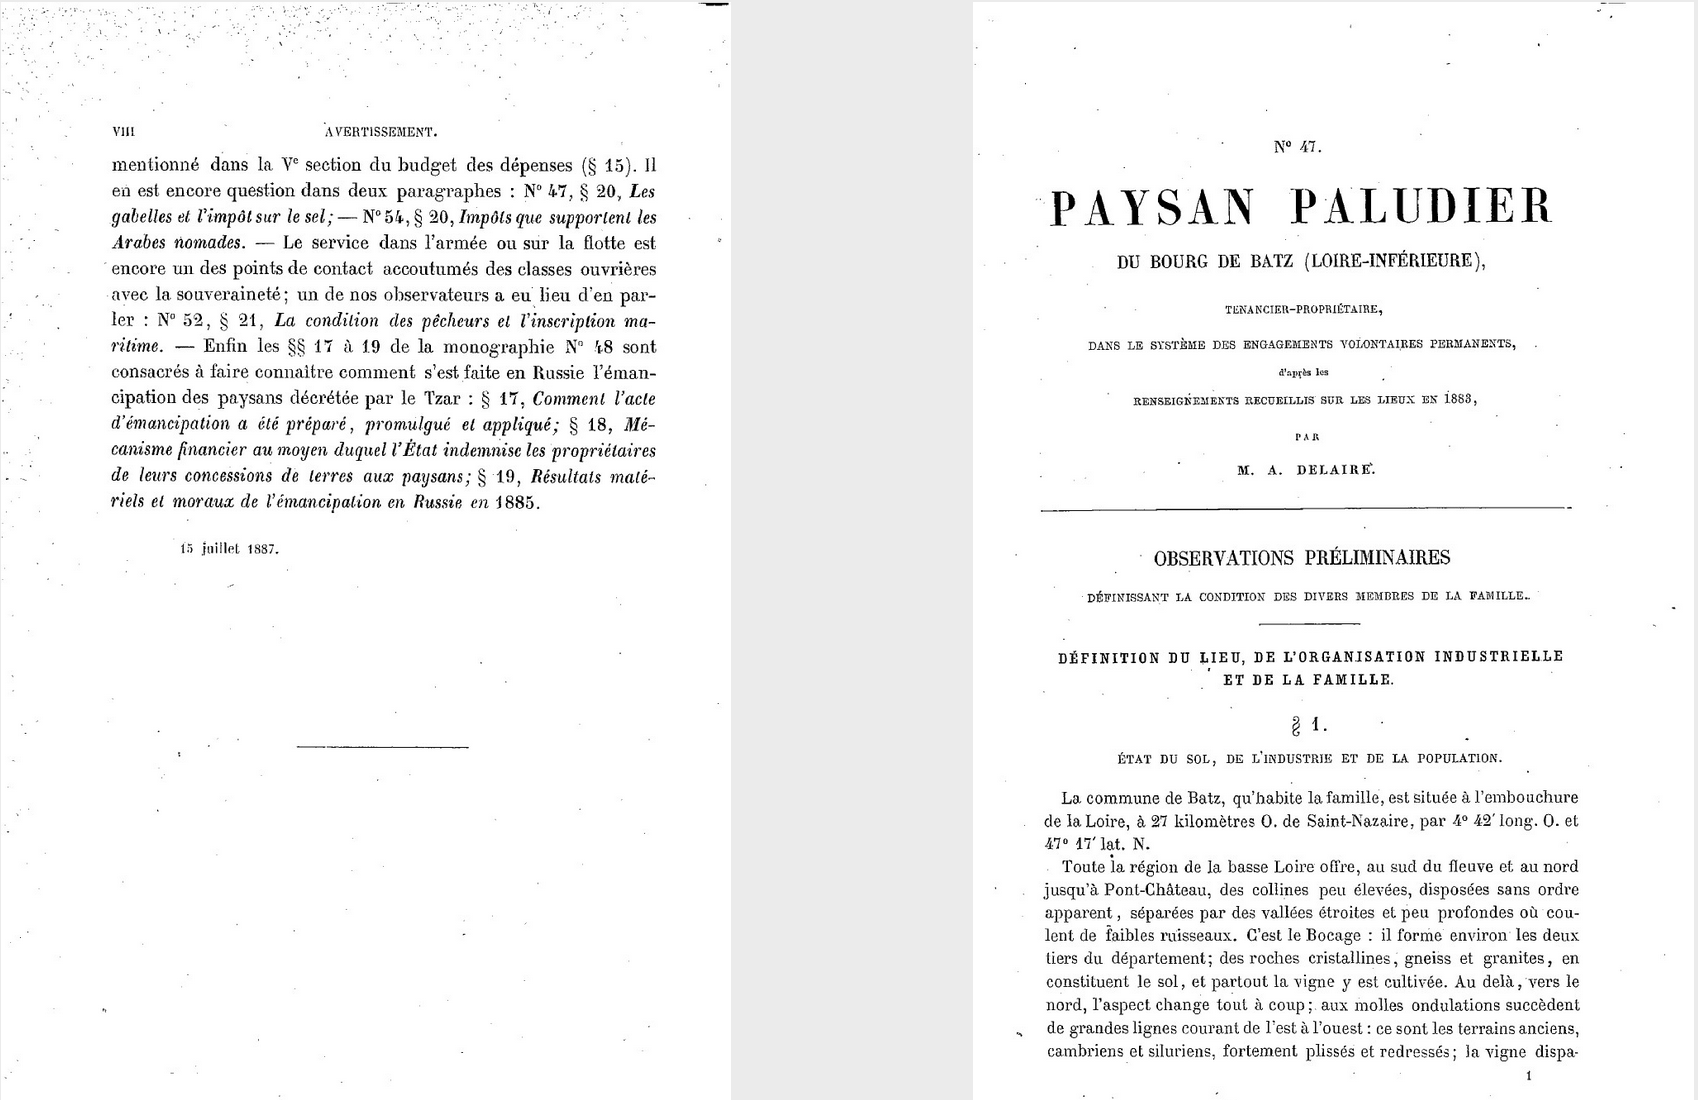
\includegraphics[width=1\linewidth]{img/odm47_bnf_1.png}
     \caption{}
     \label{odm47bnf}
    \end{subfigure}
    \caption{Comparaison des exemplaires de Toronto et de Paris. (a)~Toronto. Fin de l'\textit{Avertissement} général du volume et début du fascicule. (b)~Toronto. \textit{Avertissement} du fascicule et page de titre de la monographie. (c)~Toronto. Début de la monographie. (d)~Paris. Fin de l'\textit{Avertissement} général du volume et début de la monographie.}
    \label{odm47}
\end{figure}

Deux versions de ce même volume sont à notre disposition. L'une résulte de la numérisation de l'exemplaire déposé à Paris à la Bibliothèque nationale de France et conservé par le département Philosophie, histoire, sciences de l'homme\footnote{Consultable sur \textit{Gallica} : \url{https://gallica.bnf.fr/ark:/12148/bpt6k54465138} (consulté le \today).}, la seconde se trouve à la \textit{John P. Robarts Research Library} de l'Université de Toronto et a été numérisée par \ia\footnote{Consultable à cette adresse : \url{https://archive.org/details/s2lesouvriersdes01sociuoft} (consulté le \today).}.

Des différences de composition existent entre les volumes. Ainsi, l'exemplaire de Toronto (\fig{} \ref{odm47ia1}, \ref{odm47ia2}, \ref{odm47ia3}) comporte deux feuillets qui ne sont pas présents dans celui de Paris (\fig{} \ref{odm47bnf}). Le premier porte au recto le titre des \odm{} et au verso l'\textit{Avertissement} que nous avons cité ci-dessus en premier, le second est la page de titre du fascicule avec un verso vierge. Dans l'exemplaire de la Bibliothèque nationale, la première page de la monographie n° 47 suit la fin de l'\textit{Avertissement} général du volume.

Laisser aux propriétaires le soin de relier les fascicules pour composer le volume final revient à rompre l'unité codicologique de ce dernier, chaque nouvelle opération de reliure donnant naissance à un nouvel exemplaire. Les relieurs ont en effet pu choisir de conserver ou de ne pas conserver les pages propres aux fascicules, à l'instar des feuillets de l'exemplaire de Toronto. Il n'existe donc pas un modèle ayant autorité dans la composition des \odm{} --- en dépit du fait que les volumes de la Bibliothèque nationale de France, issus du dépôt légal, ont dû être versés par l'éditeur, \cad{} la Société internationale des études pratiques d'économie sociale.

Pour le projet \timeus{}, cela signifie que le corpus retenu pour le traitement informatisé et la publication finale ne sera qu'une version de l'\oe{}uvre que représente les \odm.

\section{Continuité et discontinuité dans la structure logique des monographies}

Un élément remarquable marque la centaine de monographies des \odm{} : une même structure logique que les éditeurs ont tenté de maintenir tout au long de la publication.

Cette structure est l'incarnation de la méthodologie le playsienne des monographies de famille.

\chapter{Des numérisations multiples}

Début du deuxième chapitre

\chapter{Un encodage automatique}

Début du troisième chapitre